\documentclass[12pt,a4paper]{article}
\usepackage[utf8]{inputenc}
\usepackage[sfdefault]{ClearSans}
\usepackage[T1]{fontenc}
\usepackage[left=35mm,right=20mm,top=25mm,bottom=25mm]{geometry}
\usepackage[czech]{babel}
\usepackage{titling}
\usepackage{graphicx}
\usepackage{caption}
\usepackage[list=true]{subcaption}
\usepackage{acronym}
\usepackage{setspace}
\usepackage{indentfirst}
\usepackage{hyperref}
\usepackage{listings}
\usepackage{tabularx}
\usepackage{changepage}

\graphicspath{ {./img/} }
\setlength{\parindent}{2em}
\setlength{\parskip}{0.1em}
\linespread{1.5}

\title{PlantHub}
\author{Filip Sikora, Jakub Vantuch}
\date{}

\begin{document}
\renewcommand*\listfigurename{}
\renewcommand{\figurename}{Obr.}
\renewcommand\refname{}

\begin{titlepage}
	\begin{adjustwidth}{-20mm}{-7.5mm} 
		\vspace*{-1.5cm}
		\noindent
\includegraphics[width=\linewidth]{header.png}
	\end{adjustwidth}
	\begin{center}
		\vspace*{0.2cm}
		\Huge\textbf{MATURITNÍ ZKOUŠKA}
		\vspace*{1cm} \\
		\large \emph{PRAKTICKÁ ZKOUŠKA Z ODBORNÝCH PŘEDMĚTŮ}
		\vspace*{1cm} \\
		\Large Téma č. 4 \\
		\vspace*{1cm}
		\Large Zavlažovací systém PlantHub \\
		\vfill
		\normalsize
	\end{center}
	\begin{tabularx}{\textwidth}{l@{\hskip 0.5cm}XXl}
		Obor vzdělání: & \multicolumn{3}{c}{\textbf{18 – 20 – M/01 Informační technologie}} \\[10pt]
		Třída: & \textbf{4. IT} & Autor práce: & \textbf{Jakub Vantuch} \\[10pt]
		Školní rok: & \textbf{2021/22} & Vedoucí učitel práce: & \textbf{Ing. Jiří Sumbal}
		\vspace*{1cm}
	\end{tabularx}
	„Prohlašujeme, že jsme tuto práci vypracovali samostatně a použili jsme literárních pramenů a informací, které citujeme a uvádíme v seznamu použité literatury a dalších zdrojů informací.“ \\
	\vspace*{0.5cm} \\
	\renewcommand{\arraystretch}{2}
	\begin{tabularx}{\textwidth}{l@{\hskip 0.75cm}X@{\hskip 1.5cm}X@{\hskip 0.75cm}l}
		Ve Frýdku-Místku, dne: & \dotfill & \dotfill & podpis \\
		Ve Frýdku-Místku, dne: & \dotfill & \dotfill & podpis \\
	\end{tabularx}
\end{titlepage}

\clearpage

\section*{Anotace}

PlantHub je zavlažovací systém, s plánovaným a automatickým způsobem zavlažování. Nastavení celého systému je možno upravit přes \ac{WUI}, které navíc nabízí i dashboard a prostředí pro manuální ovládání čerpadla. Jádrem našeho systému je mikropočítač \ac{RPi}, který slouží jako hostovací zařízení pro webový server a databázi, a zároveň jako řídící jednotka celého našeho systému. Systém PlantHub dále získává informace o vlhkosti půdy, teplotě a vlhkosti vzduchu a hladině vody, a vykresluje je ve svém \underline{\ac{WUI}}. Ve stejné chvíli naměřená data ukládá do databáze v periodě 4 hodin. Jelikož voda časem v nádrže dojde, systém PlantHub snímá stav hladiny vody v nádrži a včas upozorní, že je třeba ji doplnit.

\section*{Klíčová slova}

\noindent zavlažování; automatizace; statistika; mikropočítač; uživatelské rozhraní

\clearpage

\tableofcontents

\clearpage

\section{Úvod}

Naším cílem je návrh, sestavení a naprogramování automatického zavlažovacího systému s názvem PlantHub. Systém se skládá z řídící jednotky (stanice), senzorů, čerpadla, nádrže a \space \underline{\ac{WUI}}. Tato stanice pravidelně snímá data ze senzorů měřících teplotu a vlhkost vzduchu, vlhkost půdy a stav hladiny v nádrži, ze které stanice přečerpává vodu. Naměřená data se živě odesílají a zobrazují ve \underline{\ac{WUI}} a ve stejné chvíli se samostatně, v periodě čtyř hodin ukládají do databáze. Přístup k naměřeným datům a \underline{\ac{WUI}} má pouze uživatel lokální sítě, do které je PlantHub připojen.

\underline{\ac{WUI}} je hostované na naší stanici. Uživatel má možnost zobrazení statistik jak živě naměřených dat, tak dat historických. \underline{\ac{WUI}} také nabízí manuální kontrolu nad čerpadlem, nastavením \underline{\ac{WUI}} a samotné řídící jednotky.

Jednotlivé součásti a moduly stanice jsme vybrali podle finanční dostupnosti a adekvátních technických požadavků na přesnost měření. Obvod jsme v testovací verzi postavili na nepájivém poli a ve finální verzi navrhli a objednali vlastní \ac{PCB}. Pro ochranu naší stanice jsme navrhli kryt, který jsme následně vytiskli na 3D tiskárně.

Hlavní program jsme napsali v programovacím jazyce Go, jehož hlavní využití je vytváření backendů webových aplikací. Tento jazyk se nám zalíbil natolik že jsme se v něm rozhodli vytvořit jak \ac{API}, databázové funkce, tak i hlavní program. Program je rozdělen na několik sekvencí, z toho hlavní jsou měřící sekvence a sekvence controlleru, která pomocí snímání dat z databáze určuje, jestli se jedná o první spuštění PlantHubu, a podle toho určí jestli se spustí incializační sekvence nebo sekvence samotného zavlažování.

\clearpage

\section{Seznam zkratek a pojmů}
\begin{acronym}
	\acro{WUI}{webové uživatelské rozhraní}	
	\acro{API}{application programming interface} \\
		Spojení pro přenos dat mezi zařízeními nebo programy pomocí http protokolu.
	\acro{REST}{representaion programming interface} \\
		Definuje strukturu \underline{\ac{API}} tak, že zobrazuje všechna data a vytváří k nim jednoduchý přístup. Protože ale nenačítá pouze vybraná data, není tento proces vždy vhodný, jelikož může v mnoha případech zpomalovat celou aplikaci. 
	\acro{GraphQL}{graph query language}
	\acro{PCB}{plošný spoj}
	\acro{RPi}{Raspberry Pi}
	\acro{ADC}{analogově digitální převodník}
	\acro{DHT11}{digital humidity temperature v.11}
	\acro{HC-SR04}{Ultrasonický senzor vzdálenosti}
	\acro{LED}{light emitting diode}
	\acro{SAR}{successive-approximation}
	\acro{MSB}{most significant bit}
	\acro{LSB}{least significant bit}
	\acro{Vref}[$ V_{ref}$]{Referenční napětí}
	\acro{Vin}[$ V_{in}$]{Vstupní napětí}
	\acro{Vdac}[$ V_{dac}$]{Napětí zpětně převedené do dekadické hodnoty z poslední binární hodnoty}
\end{acronym}

\clearpage

\section{Hardware}

\subsection{Senzory}

\subsubsection{Senzor teploty a vlhkosti vzduchu DHT11}

Senzor \ac{DHT11} se skládá z jednotky pro měření teploty, jednotky pro měření vlhkosti vzduchu a převodníku.

Teplotu měří senzor termistorem. Termistor je keramický polovodič, který zmenšuje svou rezistivitu, když se okolní teplota zvýší.

Vlhkost měří senzor na základě rezistivity substrátu umístěného mezi dvěma elektrodami. Tento substrát zachytává vlhkost a vytváří tak vodivé prostředí

\subsubsection{Senzor vlhkosti půdy}

Jedná se o kapacitní senzor, který se skládá ze dvou vodivých desek a převodníku. Čidlo funguje na způsob kapacitoru avšak jeho kapacita je ovlivněna vlhkostí, která ovlivňuje dielektrikum mezi dvěma deskami.

\subsubsection{Analogově digitální převodník MCP3008}

\underline{\ac{RPi}} má v rámci general-purpose input/output (GPIO) pinů pouze digitální vstupy, protože je ale senzor vlhkosti půdy analogový museli jsme použít \ac{ADC}.

Pomocí \underline{\ac{ADC}} v integrovaném obvodu s 10-bitovým rozlišením tedy přemapujeme analogový signál do osmi různých digitálních hodnot, kterým se také říká bitové rozlišení. \underline{\ac{ADC}} měří hodnoty od 0 až po 1023 a následně je pomocí Serial Peripheral Interface (SPI) komunikace posílá do \underline{\ac{RPi}}. \underline{\ac{RPi}} metodou \ac{SAR} definuje adresu v binární formě srozumitelné pro digitální vstup. V první iteraci převodu se na \underline{\ac{SAR}} registru nastaví první bit na logickou hodnotu 1, stane se z něj \ac{MSB}, ten určuje pozici výstupu srovnávání dané iterace. Je nutné mít správné referenční napětí, to totiž určuje nejvyšší možnou binární adresu. Adresa v první iteraci teda bude polovinou nejvyšší možné binární adresy + 1. V další iteraci je první bit \ac{LSB}, to je ten bit který se v dané iteraci používá pro výstup srovnávání, a druhý bit se stává \underline{\ac{MSB}}. Srovnává se hodnota zpětné konverze binární adresy s hodnotou analogového vstupu, pokud je větší na \underline{\ac{MSB}} se nastaví logická hodnota 1, pokud menší tak logická hodnota 0. Podle počtu bitů \underline{\ac{ADC}} se určují iterace a přesnost převedené hodnoty.

Pro jednoduchost příklad se 4-bitovým \underline{\ac{ADC}}

\ac{Vref} = 16V; \ac{Vin} = 11.2V; \ac{Vdac} se v 1. iteraci rovná polovině \underline{\ac{Vref}}.

1. iterace

\begin{center}
	\begin{tabular}{ |c|c|c|c| } 
		\hline
		(\underline{\ac{MSB}}) & & & \\ 
		\hline
		1 & 0 & 0 & 0 \\ 
		\hline
	\end{tabular}
\end{center}

2. iterace

	\ac{Vdac} = 8

	\underline{\ac{Vin}} > \underline{\ac{Vdac}} => \underline{\ac{LSB}} = 1; \underline{\ac{MSB}} = 1

\begin{center}
	\begin{tabular}{ |c|c|c|c| } 
		\hline
		(\underline{\ac{LSB}}) & (\underline{\ac{MSB}}) & & \\ 
		\hline
		1 & 1 & 0 & 0 \\ 
		\hline
	\end{tabular}
\end{center}

3. iterace

	\ac{Vdac} = 12

	\underline{\ac{Vin}} < \underline{\ac{Vdac}} => \underline{\ac{LSB}} = 0; \underline{\ac{MSB}} = 1

\begin{center}
	\begin{tabular}{ |c|c|c|c| } 
		\hline
		& (\underline{\ac{LSB}}) & (\underline{\ac{MSB}}) & \\ 
		\hline
		1 & 0 & 1 & 0 \\ 
		\hline
	\end{tabular}
\end{center}

4. iterace

	\ac{Vdac} = 10

	\underline{\ac{Vin}} > \underline{\ac{Vdac}} => \underline{\ac{LSB}} = 1; \underline{\ac{MSB}} = 1

\begin{center}
	\begin{tabular}{ |c|c|c|c| } 
		\hline
		& & (\underline{\ac{LSB}}) & (\underline{\ac{MSB}}) \\ 
		\hline
		1 & 0 & 1 & 1 \\ 
		\hline
	\end{tabular}
\end{center}

% TODO: toto je prý na kokot napsané
% mr. sumbal nechápe co je SAR
% Přemapujeme tedy analogový signál do osmi různých digitálních hodnot, kterým se také říká 3bitové rozlišení, to definuje tu nejmenší hodnotu změny, který převodník dokáže rozlišit, této hodnotě se říká Least significant bit (LSB). \underline{\ac{ADC}} poté pomocí metody successive-approximation definuje adresu v binární formě srozumitelné pro digitální vstup.

% \begin{figure}[h]
% 	\centering
% 	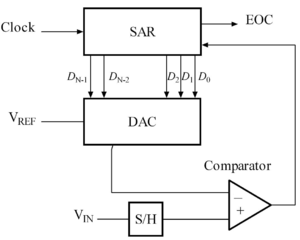
\includegraphics[width=8cm]{sar_adc.png}
% 	\caption{\ac{SAR}}
% \end{figure}

\subsubsection{Ultrasonický senzor HC-SR04}

\ac{HC-SR04} vydává zvukové vibrace na vysoké frekvenci, neslyšitelné pro lidské ucho. Poté čeká, až se zvuk odrazí zpět od překážky, a vypočítá vzdálenost na základě času měřeného od vysílání zvukové vlny k zpětnému přijmutí.

Všechny naměřené údaje jsou v převodníku senzoru přepočítány a odeslány analogovým signálem do řídící jednotky.
% TODO: převodník nepřepočítává hovno, za jak dlouho se zvuk vrátí počítá code

\subsubsection{Čerpadlo}

Námi zvolené ponorné mini čerpadlo eses se skládá z DC motoru, na němž je upevněna centrifuga pro čerpání vody a vlastního pouzdra, z kterého vede otvor pro napojení odtokové hadičky. Čerpadlo je připojeno na zdroj napětí 5V a jeho kostra je přizemněna.

\subsubsection{Tranzistor 2N2222}

Protože samotný signální pin neposkytuje dostatečné napětí pro chod čerpadla ovládáme jej tranzistorem 2N2222. Tento tranzistor je bipolární Negative-Positive-Negative tranzistor, to znamená že jeho polarita je nastavená tak aby na kolektoru přijímal pozitivní napětí. Díky našemu vyměnitelnému připojení modulů je možné čerpadlo vyměnit za jiné a přívodný kabel používat jako spouštěč čerpadla jakéhokoliv výkonu a nároků na zdroj.

\subsection{Raspberry Pi}

Vybrali jsme si jej, protože kombinuje malou velikost a vyšší výpočetní sílu než Arduino. Musí totiž zvládnout řídit všechny senzory, ukládat data do databáze a zároveň hostuje i samotnou webovou aplikaci.

\subsubsection{Architektura ARM}

Advanced RISC Machines (ARM) je založen na Reduced Instruction Set Computing (RISC) a je to nejnověji používaná CPU architektura. Tyto procesory jsou designované na všechny moderní chytré telefony, zařízení s operačním systémem Android i Apple produkty.

\subsection{Router}

Připojení \underline{\ac{RPi}} do lokální sítě je provedeno pomocí ethernet kabelu do patřičného routeru s dynamic host configuration protocol (DHCP) mechanismem. Klientský počítač připojený do stejné sítě si poté může jednoduše zobrazit \underline{\ac{WUI}} hostované na samotném \underline{\ac{RPi}}

\section{Návrh obvodu a plošného spoje}

\subsection{Testovací verze}

V prvním kroku jsme si vytvořili grafické znázornění celého obvodu (Obr. \ref{fig:graficke-znazorneni-obvodu}) v nástroji figma \cite{figma}, Testovací verzi našeho obvodu jsme postavili na nepájivém kontaktním poli. Jakmile jsme měli vše plně odzkoušeno a plně otestováno, přešli jsme na profesionálnější řešení.

\noindent\begin{figure}[h]
	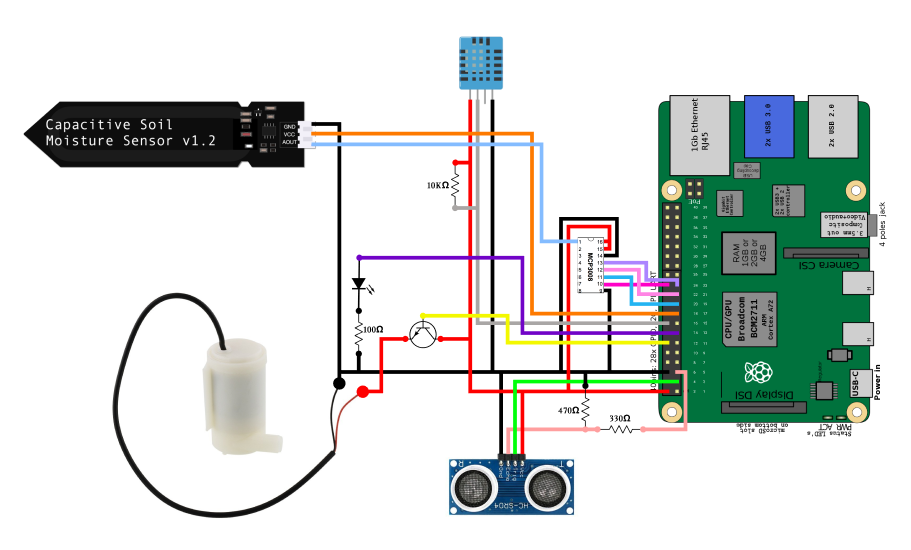
\includegraphics[width=\linewidth]{obvod.png}
	\caption{Grafické znázornění obvodu}
	\label{fig:graficke-znazorneni-obvodu}
\end{figure}

\clearpage

\subsection{Finální verze}

Ve finální verzi jsme v nástroji EasyEDA \cite{easyeda} navrhli naše vlastní schéma obvodu (Obr. \ref{fig:schema-obvodu}). Toto schéma jsme si nechali vytisknout společností JLCPCB, a po doručení jsme na něj napájeli patřičné komponenty (Obr. \ref{fig:finalni-verze}).

\vspace*{2cm}
\begin{figure}[h]
	\begin{minipage}[t]{0.5\linewidth}
		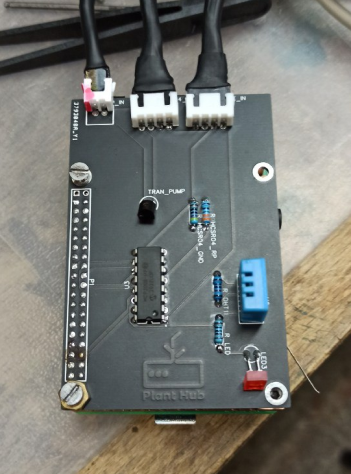
\includegraphics[width=\linewidth]{pcb.png}
		\caption{Schéma obvodu}
		\label{fig:schema-obvodu}
	\end{minipage}
	\hfill
	\begin{minipage}[t]{0.5\linewidth}
		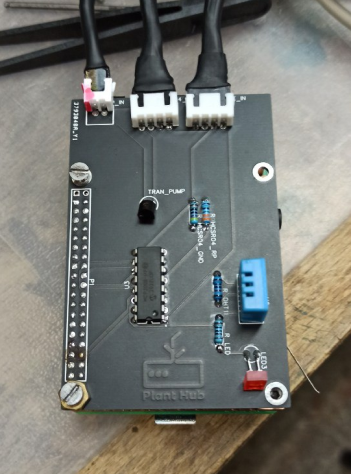
\includegraphics[width=\linewidth]{planthub.png}
		\caption{Finální verze \underline{\ac{PCB}} se senzory}
		\label{fig:finalni-verze}
	\end{minipage}
\end{figure}

%\caption{}

\clearpage

\section{Fyzická realizace}

Vymstila se nám však nepřesnost rozměrů krytu a při vkládání stanice do krytu se nám podařilo zlomit SD kartu s operačním systémem, daty a nasazenými programy. Po reinstalaci operačního systému jsme opravili rozměry vytvořeného modelu krytu a vytiskli kryt podruhé, tentokrát ve správných rozměrech.

\subsection{Pouzdro}

Navhrli jsme vhodné pouzdro pro naše \underline{\ac{RPi}}, abychom ochránili citlivé elektronické součástky a zároveň měli možnost jednoduše vyjmout stanici z krytu. Pouzdro jsme vytiskli na školní 3D tiskárně pevným Polyethylene terephthalate glycol (PETG) filamentem.

%TODO předělat na fotku pouzdra

\begin{figure}[h]
	\centering
	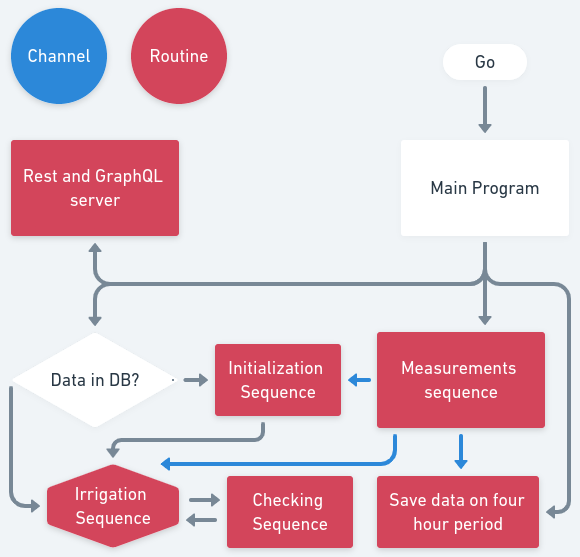
\includegraphics[width=0.72\linewidth]{go.png}
	\caption{Pouzdro}
\end{figure}

\subsection{Hub}

Zkompletovaný hub se tedy skládá z pouzdra, \underline{\ac{RPi}}, \underline{\ac{PCB}} a připojených senzorů, ethernet kabelu a zdrojového kabelu. Jednoduchým způsobem je možno hub rozebrat pro možnou opravu.

%TODO předělat na fotku hubu

\begin{figure}[h]
	\centering
	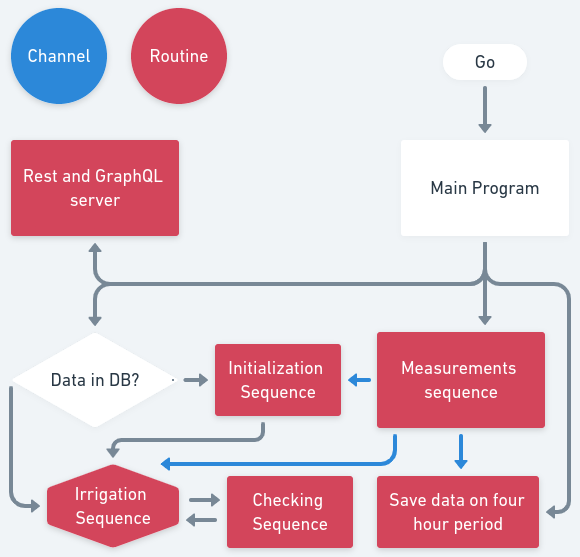
\includegraphics[width=0.72\linewidth]{go.png}
	\caption{Hub}
\end{figure}

\subsection{Nádrž}

K zavlažování bylo potřeba postavit i nádrž na vodu, ze které bude naše čerpadlo přečerpávat vodu k zavlažování. Nejvhodnější řešení byla nádoba s co největším objemem, která bude jednoduše přenosná, odolná a nebude složité připevnit na ní senzory. Nakonec jsme ji postavili z upraveného 5L pivního soudku, natřeli antikorozní barvou a upravili ji, k našim potřebám.

%TODO předělat na fotku nádrže

\begin{figure}[h]
	\centering
	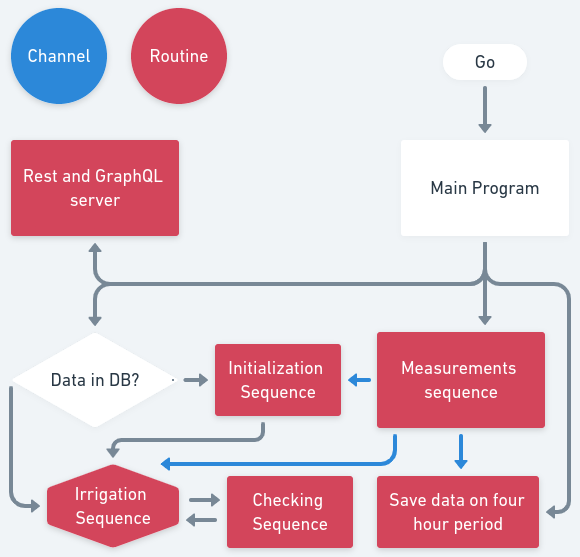
\includegraphics[width=0.72\linewidth]{go.png}
	\caption{Nádrž}
\end{figure}

\subsection{Celý systém}

%TODO předělat na fotku celého planthubu

\begin{figure}[h]
	\centering
	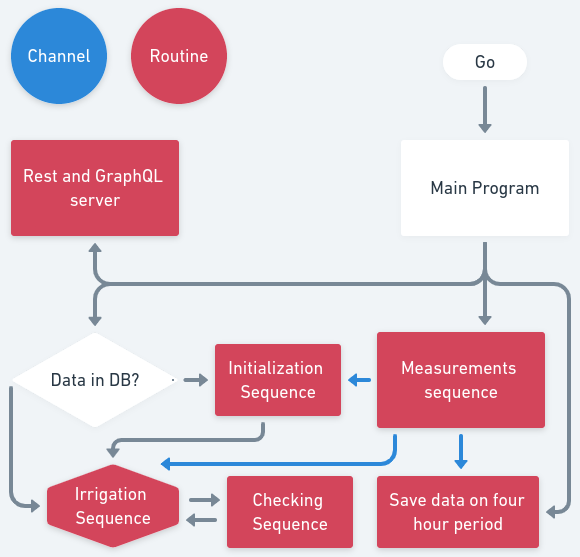
\includegraphics[width=0.72\linewidth]{go.png}
	\caption{Fyzická realizace}
\end{figure}

\clearpage

\section{Hlavní program}

\subsection{Postup práce}

Náš hlavní program pro zavlažování a komunikaci s databází a \underline{\ac{WUI}} jsme začali psát ve vysokoúrovňovém programovacím jazyce Python. Od toho jsme ale nakonec upustili kvůli horší výkonu, a tak jsme program přepsali v programovacím jazyku Go.

\begin{figure}[h]
	\centering
	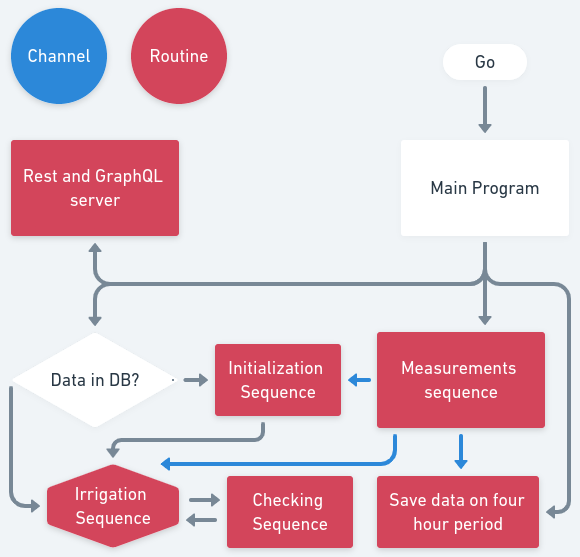
\includegraphics[width=0.72\linewidth]{go.png}
	\caption{Vývojový diagram programu}
\end{figure}

\subsection{Fáze programu}

Fáze programu se spouštějí buďto v samostatné go rutině a komunikují spolu pomocí kanálů nebo na základě podmínek, kde se po splnění požadavků ukončí.

\subsubsection{Měření}

Senzor vlhkosti půdy a \underline{\ac{DHT11}} průběžně posílají naměřená data do \underline{\ac{WUI}}. Hlavní program ve stejné chvíli čte data ze senzorů a kontroluje jestli naměřené hodnoty nepřekračují limitní hodnoty pro spuštění zavlažování, pokud ano \underline{\ac{RPi}} pošle signál pro otevření tranzistoru což spustí čerpadlo.

\subsubsection{Periodické ukládání dat}

V samostatné rutině běží funkce pro ukládání naměřených dat v periodě 4 hodin. Tato rutina, stejně jako ostatní, čte hodnoty senzorů z měřící sekvence. Naměřená data jsou následně statisticky zobrazena ve \underline{\ac{WUI}}.

\subsubsection{Controller}

Po spuštění měřící sekvence a sekvence periodického ukládání dat se spustí buďto inicializační sekvence a nebo zavlažovací sekvence podle toho, jestli se v databázi nachází předchozí nastavení. Pokud předchozí nastavení nejsou nalezena, program čeká na uložení dat z \space \underline{\ac{WUI}} a \ac{LED} bliká dvakrát po sobě, dokud data nejsou dostupná. Pokud jsou, spustí se zavlažovací sekvence, načtou se limitní data z databáze a v periodě jedné sekundy se budou číst data o vlhkosti půdy.

\subsubsection{Inicializace}

Půda musí být ze začátku suchá. Senzor vlhkosti půdy zasuneme co nejhlouběji do půdy. \underline{\ac{RPi}} bude chvíli sbírat data a pak je zprůměruje do hodnoty, která bude sloužit jako limit pro spuštění čerpadla.

Ve \underline{\ac{WUI}} jde navíc ještě manuálně nastavit hranice vlhkosti půdy pro spuštění čerpadla.

Nastavit se dá také množství vody, které bude přečerpáno při jednom spuštění a jaká je hranice pro přijatelnou výšku hladiny vody v nádrži. Pokud nejsou tyto hodnoty uvedeny čerpadlo bude vodu přečerpávat, dokud se nezmění hodnota kapacitního čidla pro měření vlhkosti půdy a \space \underline{\ac{HC-SR04}} použije výchozí nastavení.

\subsubsection{Zavlažování}

Čerpadlo začne čerpat vodu a zavlažovat rostlinu. Voda se čerpá tak dlouho, dokud senzor vlhkosti půdy nezmění svou hodnotu nebo dokud není vyčerpán limit přečerpané vody na jedno spuštění.

\subsubsection{Kontrola}

Po ukončení přečerpávání se spustí \underline{\ac{HC-SR04}} a změří výšku hladiny vody. Naměřená data poté odešle do \underline{\ac{RPi}} kde se uloží do databáze. Pokud bude naměřená hodnota nižší, než je limitní hodnota, začne blikat \underline{\ac{LED}} a \underline{\ac{RPi}} odešle upozornění o doplnění nádrže do \underline{\ac{WUI}}. Jakmile bude hladina doplněna, signalizace se vypne.

\subsubsection{Ukládání dat}

Náš systém ukládá zvlášť periodicky naměřená data a data naměřená před zavlažováním, dále ukládá nastavení jak pro limity k zavlažování, tak pro \underline{\ac{WUI}}.

\subsection{Programovací jazyk Go}

Go je open-source programovací jazyk, který byl vytvořen společností Google v roce 2009. Je to stále relativně nový programovací jazyk, který se nevyvinul z jiných jazyků jako C\# a Java. Go ignoruje teorii o programovacích jazycích. Místo toho aby se zaměřoval na akademické teorie, se zaměřuje na reálné praktiky používané pro vývoj next-gen v cloudových, distribuovaných a souběžných aplikacích.

Jazyk Go je staticky typovaný a využívá garbage collector, jedná se o kompilovaný programovací jazyk, který své binární soubory kompiluje pro každou platformu. Dá se zařadit do skupiny C jazyků na základě jeho základního syntaxe. Go poskytuje expresivní syntax s jednoduchým typovým systémem a má vestavěné nástroje pro paralelní programování. Výkon Go je srovnatelný s jazyky C a C++, ale zároveň nabízí rychlý a jednoduchý vývoj aplikací.

Stejně jako C a C++ se Go kompiluje do nativního strojového kódu, takže
nepotřebujeme běhové prostředí jako Common Language Runtime (CLR) a Java Virtual Machine (JVM). To má řadu výhod, třeba při distribuci aplikace v aplikačních kontejnerech jako je Docker.

\subsubsection{Paralelní programování v Go}

Vývoj počítačů se v průběhu posledního desetiletí značně posunul. V minulosti aplikace běžely na počítačích pouze s jediným procesorovým jádrem. Dnes je standardní vidět čtyřjádrové procesory v uživatelských počítačích, dokonce i naše \underline{\ac{RPi}} má dvě jádra. Stále ale používáme programovací jazyky a technologie navržené v éře, kdy byly dostupné pouze jednojádrové procesory.

Většina programovacích jazyků dnes nabízí knihovny nebo frameworky pro \linebreak paralelní programování, ale nemají tuto vlastnost zbudovanou přímo v jádře jazyka. V Go je paralelní programování součástí jazyka už od samotného počátku. Používá takzvané Gorutiny, které umožňují spouštět funkce souběžně. Souběžné funkce pak mezi sebou mohou komunikovat a předávat data pomocí kanálů. Dokonce i některé standardní knihovny jazyka mají zabudovanou souběžnost. Například standardní knihovna `net/http' pro programování HTTP zpracovává přicházející požadavky souběžně pomocí Gorutin.

\subsubsection{Typový systém}

Pragmatický design Go neobsahuje klíčové slovo pro třídu a jeho objektová orientace je odlišná od tradičních objektově orientovaných programovacích jazyků. V Go nahrazuje funkci tradiční třídy typ struct. Dědění není v go podporováno, ale podporuje kompozici typů (Příloha 1).

\clearpage

\section{WUI}

\subsection{Programování WUI}

Webovovou aplikaci jsme napsali pomocí javascriptového frameworku
React.js, CSS frameworku Tailwind a programovacího jazyku Typescript, který je supersetem javascriptu, podporujícím volitelné statické typování. Ve webovém rozhraní je možné zobrazit si statisky jak živě naměřených dat, tak dat uložených v databázi. Z OpenWeather \underline{\ac{API}} získáváme data o předpovědi počasí a do dahsboardu renderujeme předpovědi na dalších 15h.

\subsection{Inicializační formulář}

\begin{figure}[h]
	\centering
	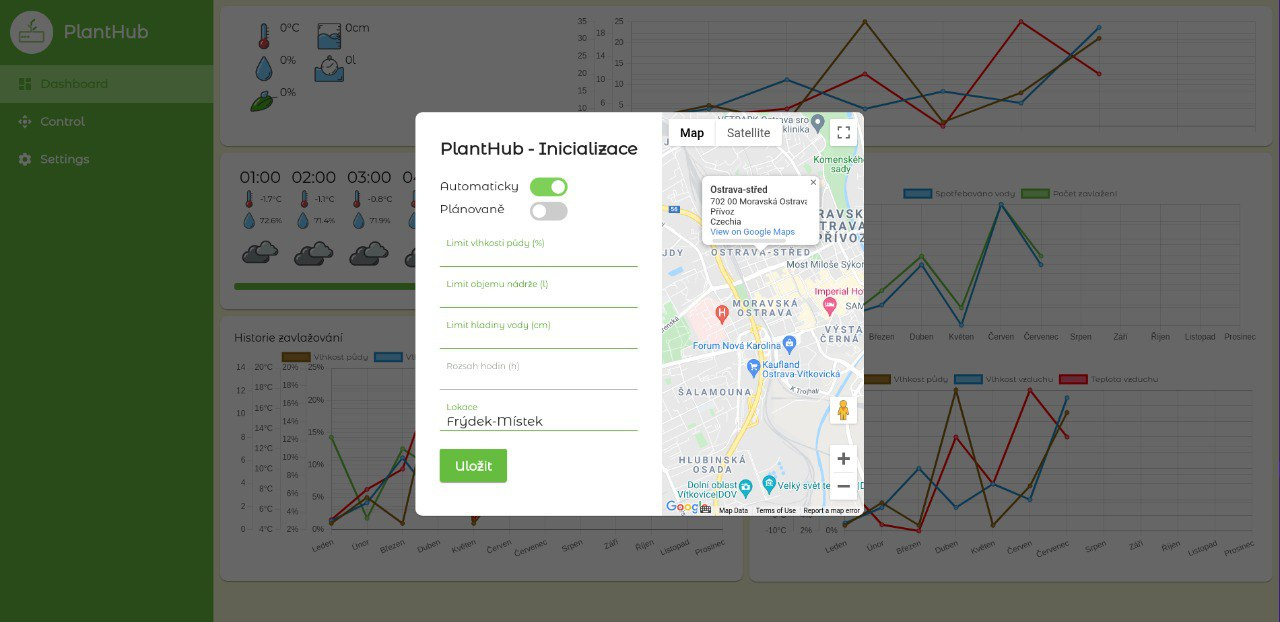
\includegraphics[width=\linewidth]{ui-inicializace.jpg}
	\caption{Inicializační formulář}
\end{figure}

Okno prvotního nastavení. Nastaví se zde limity a celkové nastavení aplikace.

\subsection{Dashboard}

\begin{figure}[h]
	\centering
	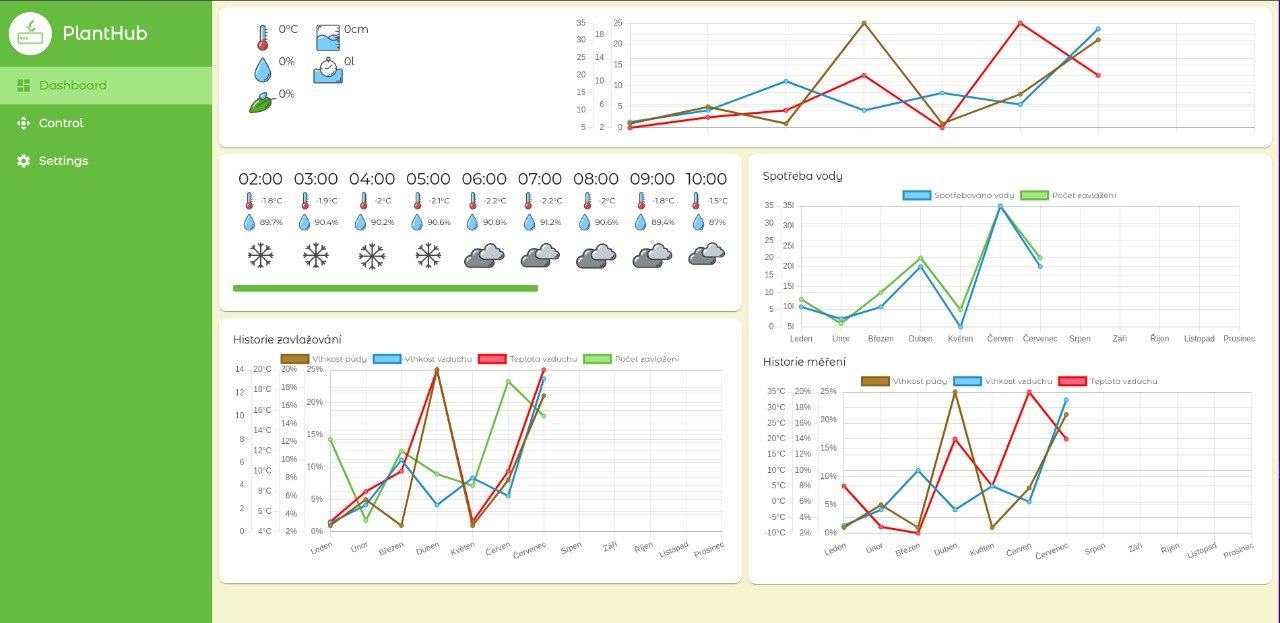
\includegraphics[width=\linewidth]{web-ui.png}
	\caption{Dashboard}
\end{figure}

\subsection{Manuální ovládání}

\begin{figure}[h]
	\centering
	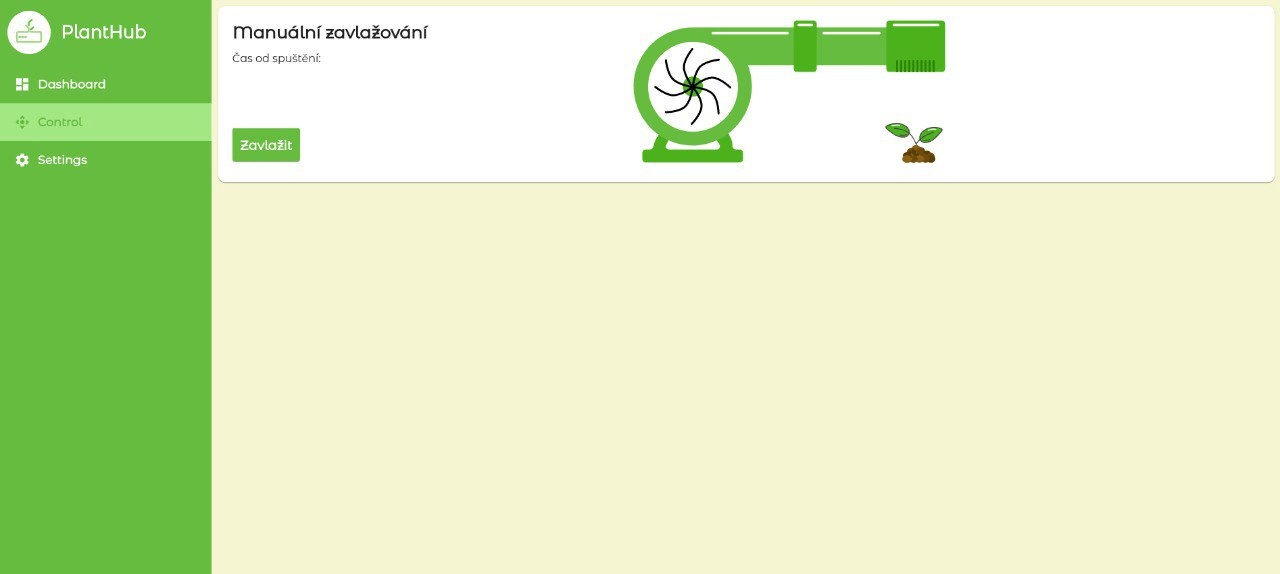
\includegraphics[width=\linewidth]{web-ui-pump.png}
	\caption{Manuální ovládání}
\end{figure}

Manuální ovládání čerpadla dovoluje uživateli kdykoliv spustit zavlažování, i po dokončení manuálního zavlažování se spustí kontrola hladiny vody v nádrži. Při úpravě limitních hodnot či jiných nastevení řídící jednotky je nutno zařízení restartovat. K tomu v sidebaru \underline{\ac{WUI}} slouží možnost "Restart HW".

\subsection{Nastavení}

\begin{figure}[h]
	\centering
	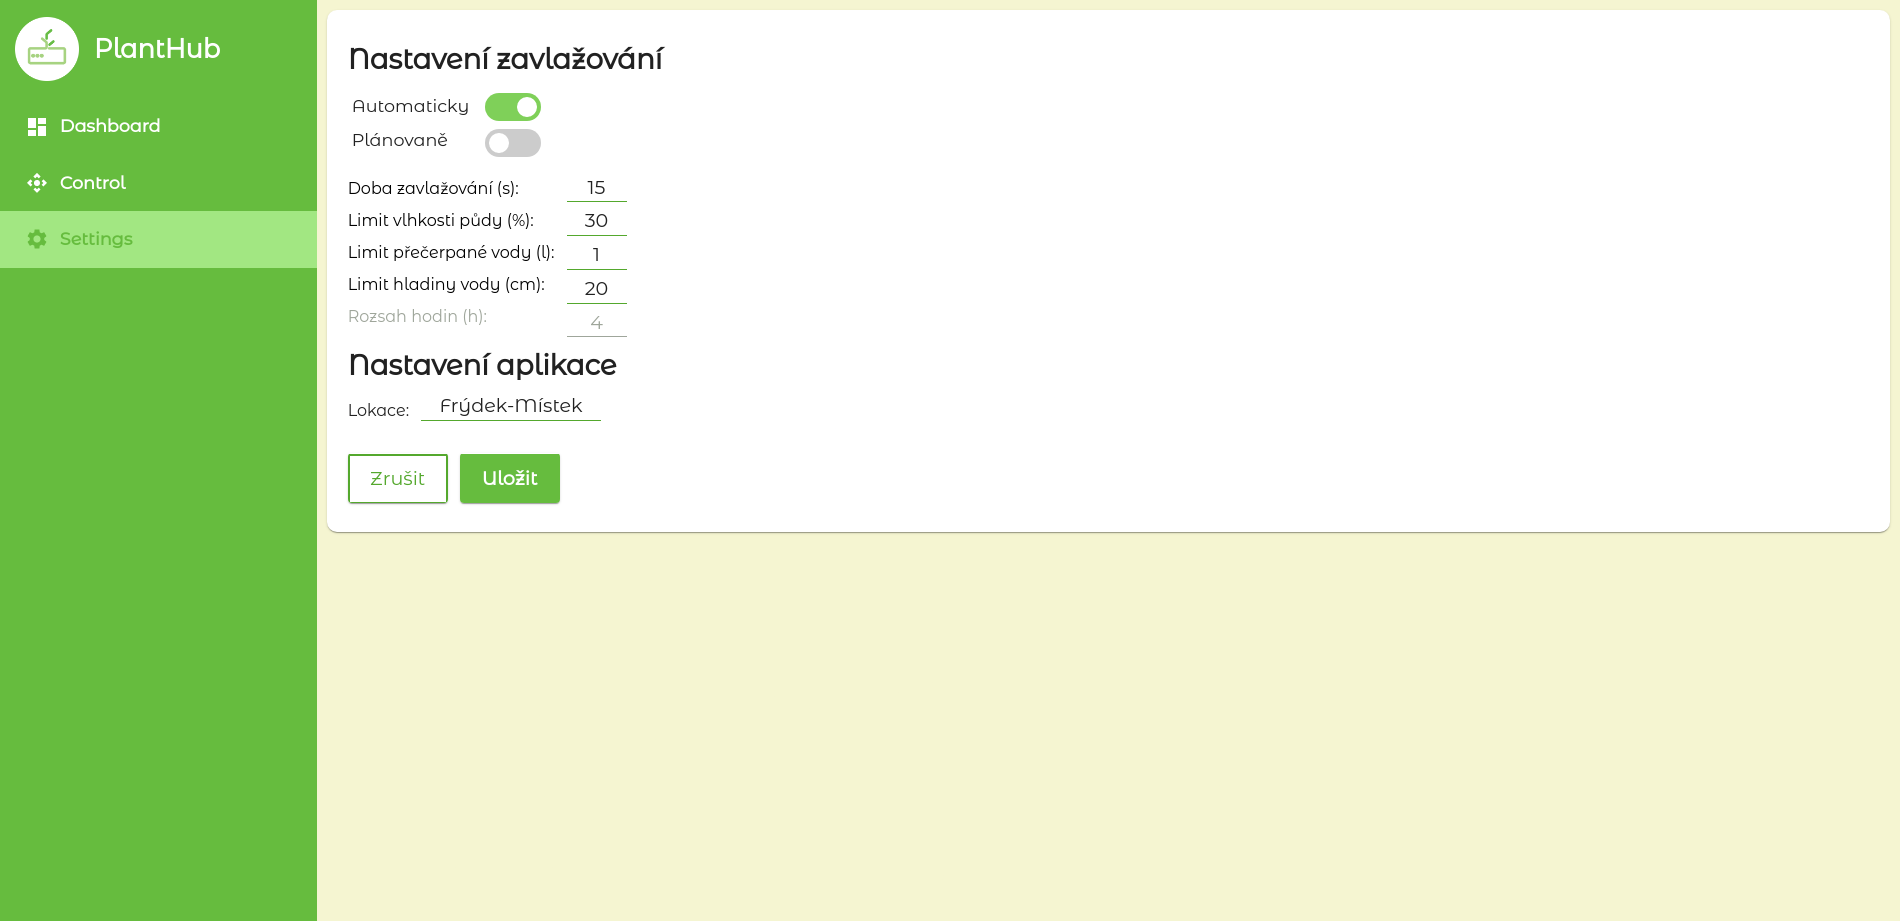
\includegraphics[width=\linewidth]{web-ui-settings.png}
	\caption{Nastavení}
\end{figure}

V nastavení se dá změnit nastavení aplikace i limitů pro zavlažování. Nastavení se poté uloží do databáze.

\subsection{Notifikace}

\clearpage

\section{Databáze}

\subsection{SQL}

Pro databázi jsme se rozhodli použít databázový systém PostgreSQL.\@ Jak vyplývá z názvu, jedná se o Structured Query Language (SQL) databázi, ty jsou vhodné pro ukládání velkého objemu dat, jako právě data z našich senzorů. Webová aplikace používá pro přístup k datům z databáze \ac{GraphQL} \space \underline{\ac{API}}.\@

\subsection{GraphQL}

Jedná se o typ přenosu dat z možností filtrace a dotazovací funkcionality. V mnoha ohledech je to konkurent řešení přenosu dat pomocí \ac{REST} \space \underline{\ac{API}}.\@ Nabízí rychlejší tvorbu \underline{\ac{API}} \space a také umožňuje efektivnější přístup k datům z databáze. Umožňuje vybrat pouze data, která momentálně aplikace používá a dovoluje vynechat data, která zrovna potřebné nejsou.

\subsection{Schéma databáze}

\begin{figure}[h]
	\centering
	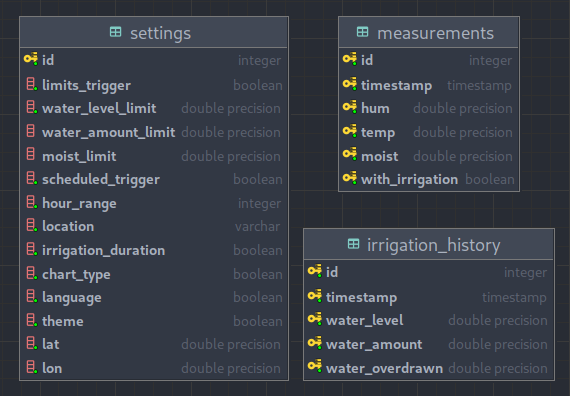
\includegraphics[width=0.9\linewidth]{db.png}
	\caption{Schéma databáze}
\end{figure}

\section{Webový server}

Web server jsme napsali v moderním jazyku Go, který nyní roste v popularitě hlavně mezi cloudovými vývojáři a v oblasti vývoje microservices. Dokáže se v rychlosti provedení programu přiblížit k nízkoúrovňovým jazykům jako je C nebo Rust, ale zároveň zůstává velmi lidsky čitelný a jednoduchý na použití. Na rozdíl od jazyků jako C a Rust má například garbage collector, který periodicky čistí paměť a zabraňuje memory leakům.

\section{Docker a kontejnerizace}

\section{Bezpečnost}

\clearpage

\section{Závěr}

Náš projekt je stále ve vývoji a některé z funkcí projektu nefungujou podle našich představ, i přes to, je náš systém v této chvíli použitelný. Myslíme si, ale že tento projekt má v budoucnu potenciál stát se úspěšným startupem, proto plánujeme pokračovat ve vývoji i po maturitě. 

Abychom však tento projekt mohli pojmout jako plně funkční systém museli bychom ještě dokončit a předělat některé klíčové části. Jednalo by se především o rozdělení hostingu webové aplikace a databáze na samostatný server a zajištění modulárnosti celého systému rozdělením řídící jednotky na samostatné moduly a hub zodpovědný za jejich provoz. V dalších, né natolik prioritních, krocích se můžeme bavit o dokončení plánované tmavé verze \underline{\ac{WUI}} a přidání podpory více jazyků. A pro odlišení od konkurence mnoha jiných zavlažovacích systémů, přidání chytrých funkcí vypočítávání spotřeby vody a energie na základě předpovědi počasí typu kytky a oblasti. 

Tato práce byla pro nás velkým přínosem, naučili jsme se mnoho nových dovedností a načerpali nové informace, které v naší profesi bezpochyby dále využijeme.

\clearpage

\section{Použitá literatura další zdroje }

\begin{thebibliography}{9}
	\vspace*{-1.5cm}
	\bibitem{texbook}
	“Home,” LaTeX, 06-May-2021. [Online]. Dostupné z: \underline{\href{https://latex-tutorial.com/}{https://latex-tutorial.com/}}. [Zpřístupněno: 10-Dubna-2022]. 

	\bibitem{golang}
	“Build fast, reliable, and efficient software at scale,” Go. [Online]. Dostupné z: \underline{\href{https://go.dev/}{https://go.dev/}}. [Zpřístupněno: 10-Dubna-2022]. 

	\bibitem{react}
	“React – a JavaScript library for building user interfaces,” – A JavaScript library for building user interfaces. [Online]. Dostupné z: \underline{\href{https://reactjs.org/}{https://reactjs.org/}}. [Zpřístupněno: 10-Dubna-2022]. 

	\bibitem{tailwindcss}
	“Rapidly build modern websites without ever leaving your HTML.,” Tailwind CSS. [Online]. Dostupné z: \underline{\href{http://www.tailwindcss.com/}{http://www.tailwindcss.com/}}. [Zpřístupněno: 10-Dubna-2022]. 

	\bibitem{typescript}
	“JavaScript with syntax for types.,” TypeScript. [Online]. Dostupné z: \underline{\href{http://www.typescriptlang.org/}{http://www.typescriptlang.org/}}. [Zpřístupněno: 10-Dubna-2022]. 

	\bibitem{vscode}
	Microsoft, “Visual studio code - code editing. redefined,” RSS, 03-Nov-2021. [Online]. Dostupné z: \underline{\href{https://code.visualstudio.com/}{https://code.visualstudio.com/}}. [Zpřístupněno: 10-Dubna-2022]. 

	\bibitem{goland}
	“Goland by jetbrains: More than just A go ide,” JetBrains. [Online]. Dostupné z: \underline{\href{https://www.jetbrains.com/go/}{https://www.jetbrains.com/go/}}. [Zpřístupněno: 10-Dubna-2022]. 

	\bibitem{git}
	Git. [Online]. Dostupné z: \underline{\href{https://git-scm.com/}{https://git-scm.com/}}. [Zpřístupněno: 10-Dubna-2022]. 

	\bibitem{figma}
	“The Collaborative Interface Design Tool.,” Figma. [Online]. Dostupné z: \underline{\href{https://www.figma.com/}{https://www.figma.com/}}. [Zpřístupněno: 10-Dubna-2022]. 

	\bibitem{freecad}
	“Freecad,” FreeCAD. [Online]. Dostupné z: \underline{\href{https://www.freecadweb.org/}{https://www.freecadweb.org/}}. [Zpřístupněno: 10-Dubna-2022]. 

	\bibitem{easyeda}
	Supplyframe, “EasyEDA,” Component Search Engine. [Online]. Dostupné z: \underline{\href{https://componentsearchengine.com/library/easyeda}{https://componentsearchengine.com/library/easyeda}}. [Zpřístupněno: 10-Dubna-2022]. 
\end{thebibliography}

\section{Seznam obrázků}

\vspace*{-1.5cm}
\listoffigures

\section{Seznam příloh}

\begin{itemize}
	\item Příloha 1: Typový systém v Go.png
	\item Příloha 2: Zdrojový kód
	\item Příloha 3: Modely krytu
	\item Příloha 4: Prezentace.pdf
\end{itemize}

\end{document} 